\documentclass{article}

\usepackage[margin=3cm]{geometry}
\usepackage{amsmath}
\usepackage{amsfonts}
\usepackage{amssymb}
\usepackage{amscd}
\usepackage{standalone}
\usepackage{float}
\usepackage{color}
\usepackage[shortlabels]{enumitem}
\usepackage{graphicx}
\usepackage{caption}
\usepackage[ngerman]{babel}
\usepackage{lscape}
\usepackage{cancel}
\usepackage{dirtytalk}
\usepackage{siunitx}
\usepackage{listings}

\graphicspath{ {./images/} }

\begin{document}
\begin{titlepage}
    \centering
    {\scshape\LARGE Hochschule für Technik und Wirtschaft Dresden \par}
    \vspace{1cm}
    {\scshape\Large Softwaresystem \glqq GPS-Track-App\grqq\par}
    \vspace{1.5cm}
    {\huge\bfseries Nutzeranleitung\par}
    \vspace{2cm}
    {\Large\itshape Raphael Neubert, Alex Schechtel, Aleksandr Pronin... \par}
    \vfill

    {\large \today\par}
\end{titlepage}

\tableofcontents
\newpage

\section{Aufnahme eines GPS-Tracks}
\section{Bearbeiten eines GPS-Tracks}
\subsection{Hinzufügen von Special Points of Interest}
\newpage
\section{GPS-Tracks mit Server synchronisieren}
    Um Ihrer  GPS-Track App den Austausch von GPS-Daten zu ermöglichen, müssen Sie das Synchronisation mit dem Server ausführen.
    \\\textbf{Wichtig:} Für eine erfolgreiche Synchronisierung ist eine Internetverbindung erforderlich.
    \begin{enumerate}
        \item Navigieren Sie zu Startseite und tippen Sie auf den Button \glqq Menu"\\
        \begin{figure}[H]
            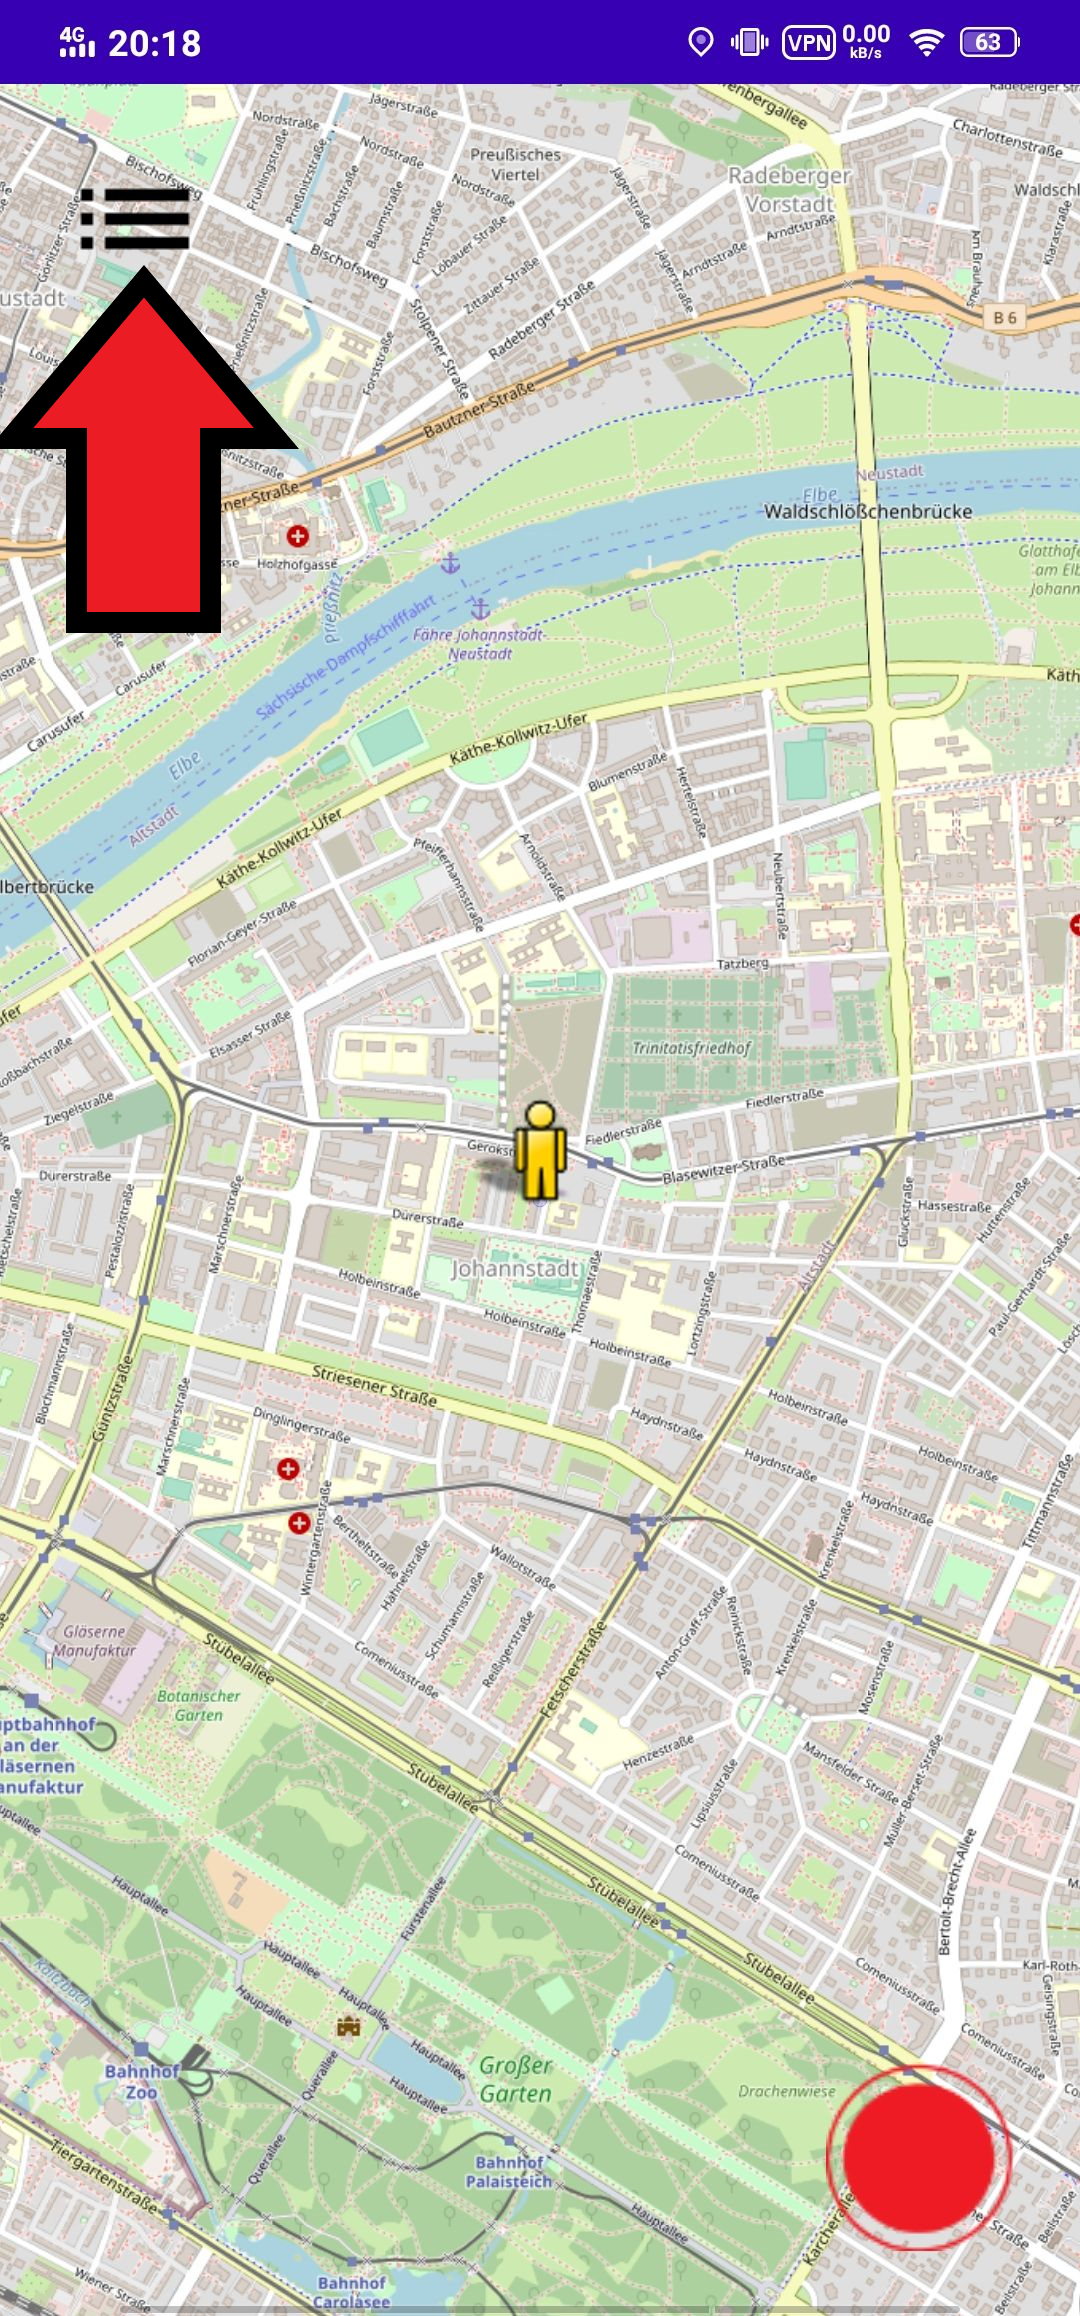
\includegraphics[scale=0.15]{1.png}
            \centering
            \caption{Menü-Button (Startseite)}
        \end{figure}
        \item Tippen Sie im erscheinenden Menü oben auf \glqq Sync" 
        \begin{figure}[H]
            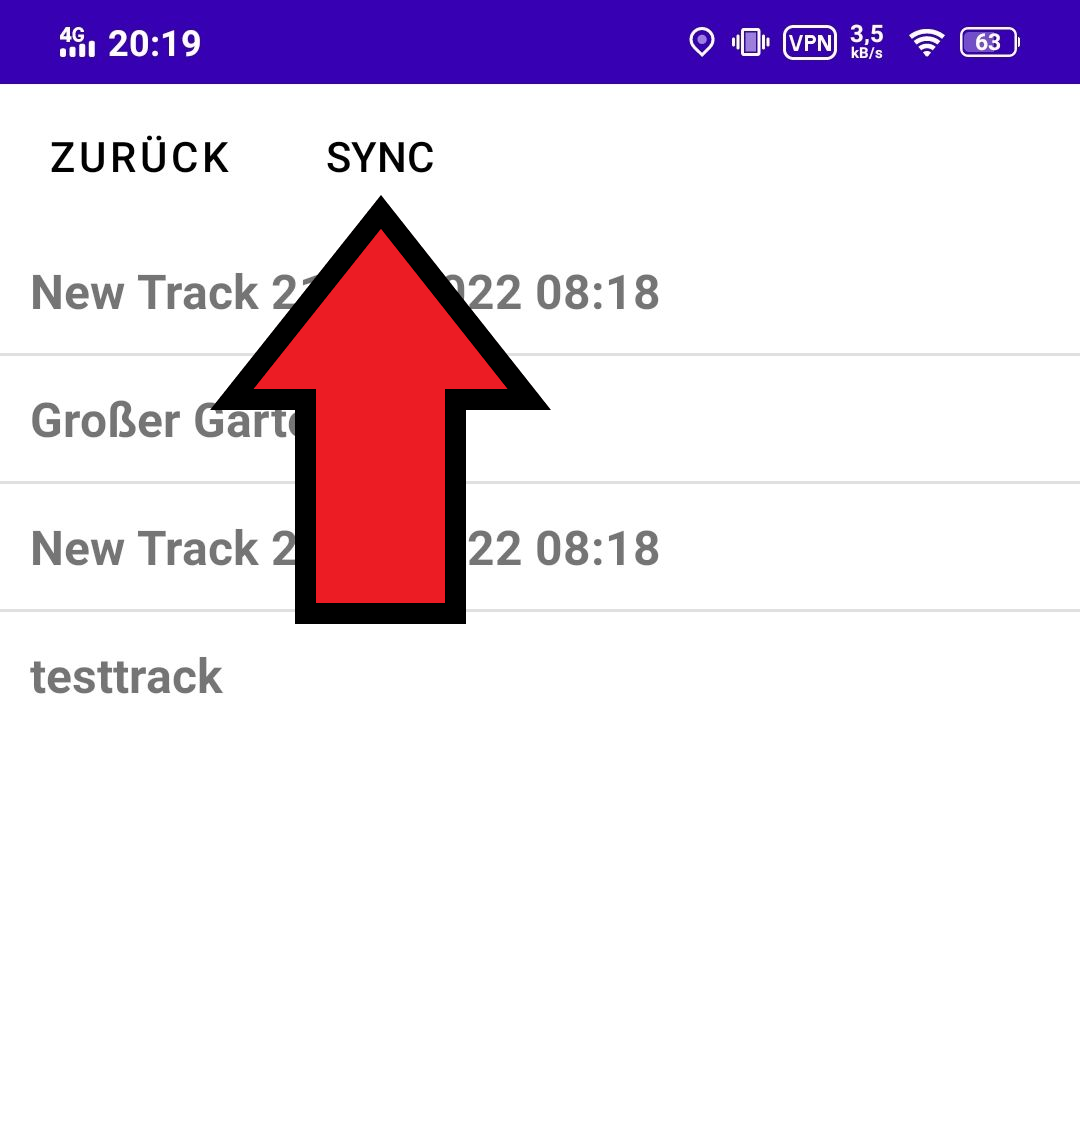
\includegraphics[scale=0.15]{2.png}
            \centering
            \caption{Sync-Button (Menüseite)}
        \end{figure}
        \item Wenn Ihre GPS-Track App mit dem Internet verbunden ist, sollte innerhalb weniger Sekunden eine
         Ladeanimation erscheinen.
        \\\textbf{Tipp:} Wenn die Ladeanimation länger als 15 Sekunden stehen bleibt, liegt möglicherweise ein Verbindungsproblem mit dem Server vor.
        \begin{figure}[H]
            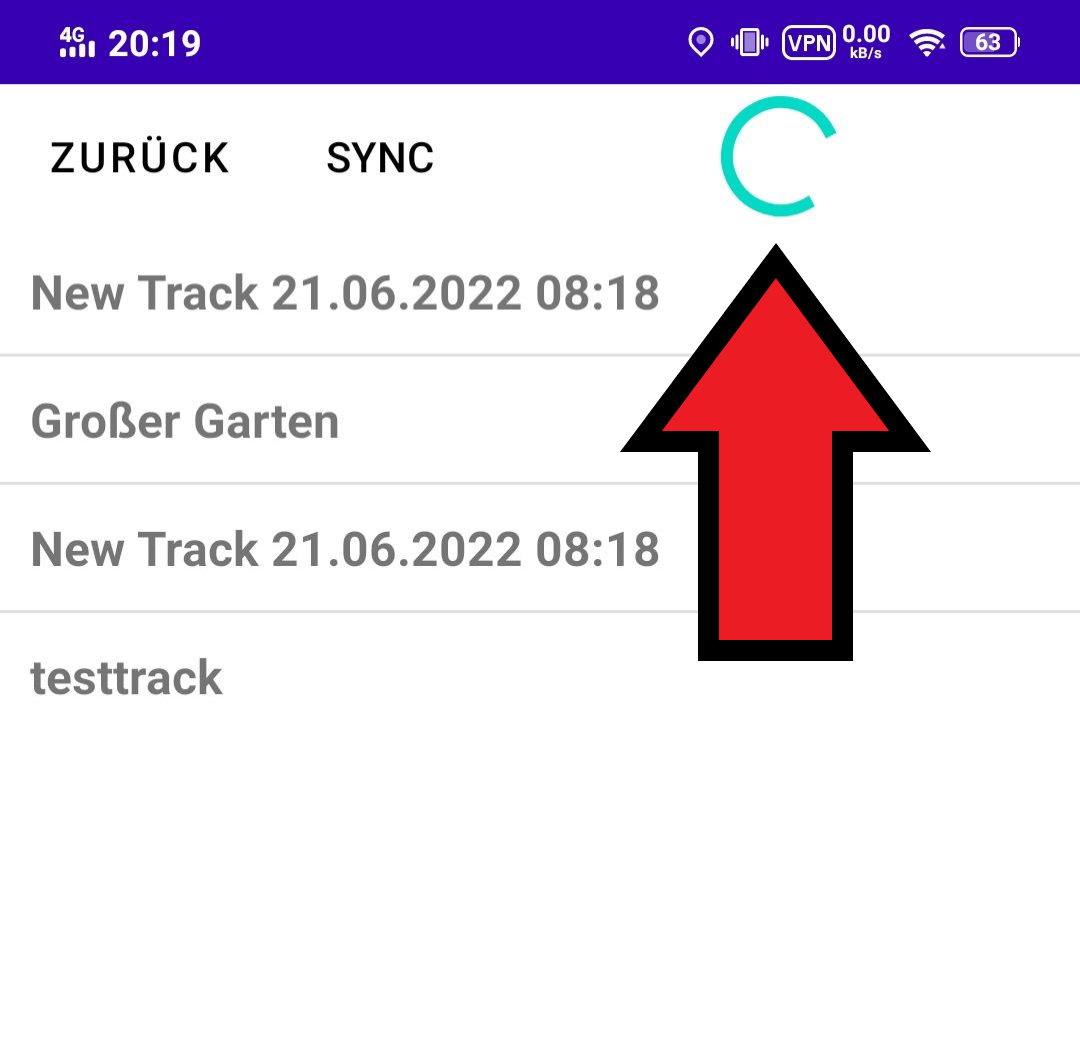
\includegraphics[scale=0.15]{3.png}
            \centering
            \caption{Ladeanimation (Menüseite)}
        \end{figure}
        \item Ihre GPS-Track App ist nun erfolgreich mit dem Server synchronisiert worden.
        \\\\\textbf{Tipp:}Wenn nach der Synchronisierung mehrere Dateien mit demselben Namen exestieren, bedeutet dies, dass die Dateien von anderen Benutzern der App bearbeitet wurden und neue Datei-IDs erhalten haben.
       \begin{figure}[H]
            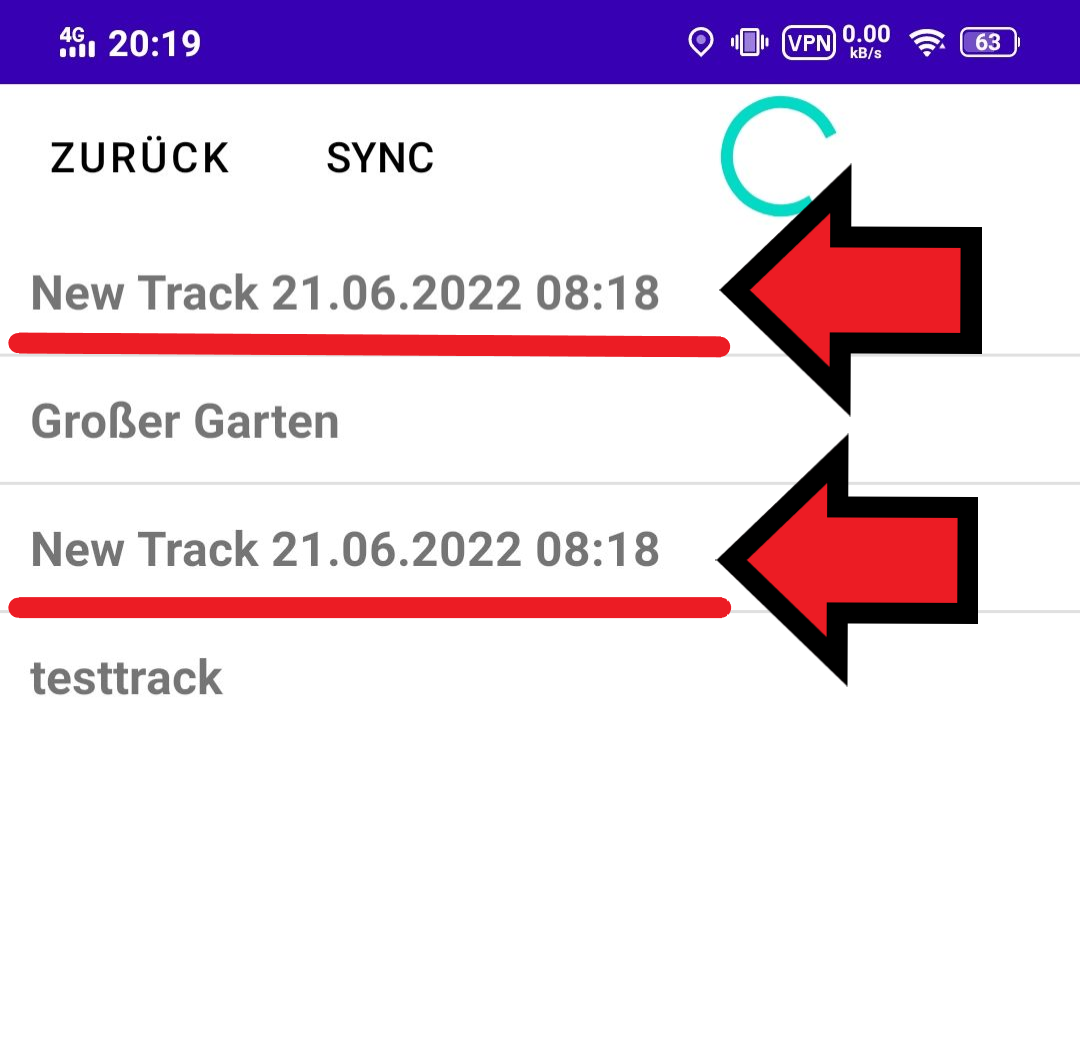
\includegraphics[scale=0.15]{4.png}
            \centering
            \caption{Dateien mit demselben Namen (Menüseite)}
        \end{figure}
    \end{enumerate}

\section{Nebenfunktionalitäten}
\subsection{GPS-Track auf Karte anzeigen}
\subsection{Details eines GPS-Tracks anzeigen}
\subsection{Aufnahme fortsetzen}
\subsection{GPS-Track umbenennen}
\subsection{GPS-Track löschen}
\end{document}
